\chapter[Optical color MIMO: Metameric modulation]{Metameric modulation}
\label{chapter:metameric}
\thispagestyle{myheadings}
%\section{Metameric modulation}
%\label{sec:metameric}
\graphicspath{{_MIMOColor/figures_mm/}}
In this chapter, we propose metameric modulation\footnote{This work is published in peer--reviewed IEEE proceeding \cite{but12a}.} - a novel modulation scheme for VLC which can maintain constant perceived ambient lighting. By using $D > 3$ LEDs, it is possible to render same illumination chromaticity with different combinations of LEDs. These different illumination SPDs are indistinguishable to humans but are distinguishable to an electronic receiver and can be achieved due to principle of metamerism. Information is encoded in changes between these states and can be recovered by detecting intensity modulation in different wavelength bands.

\section{Metamerism}
\label{subsec:metamericEye}
\begin{figure}[!t]
	\centering
    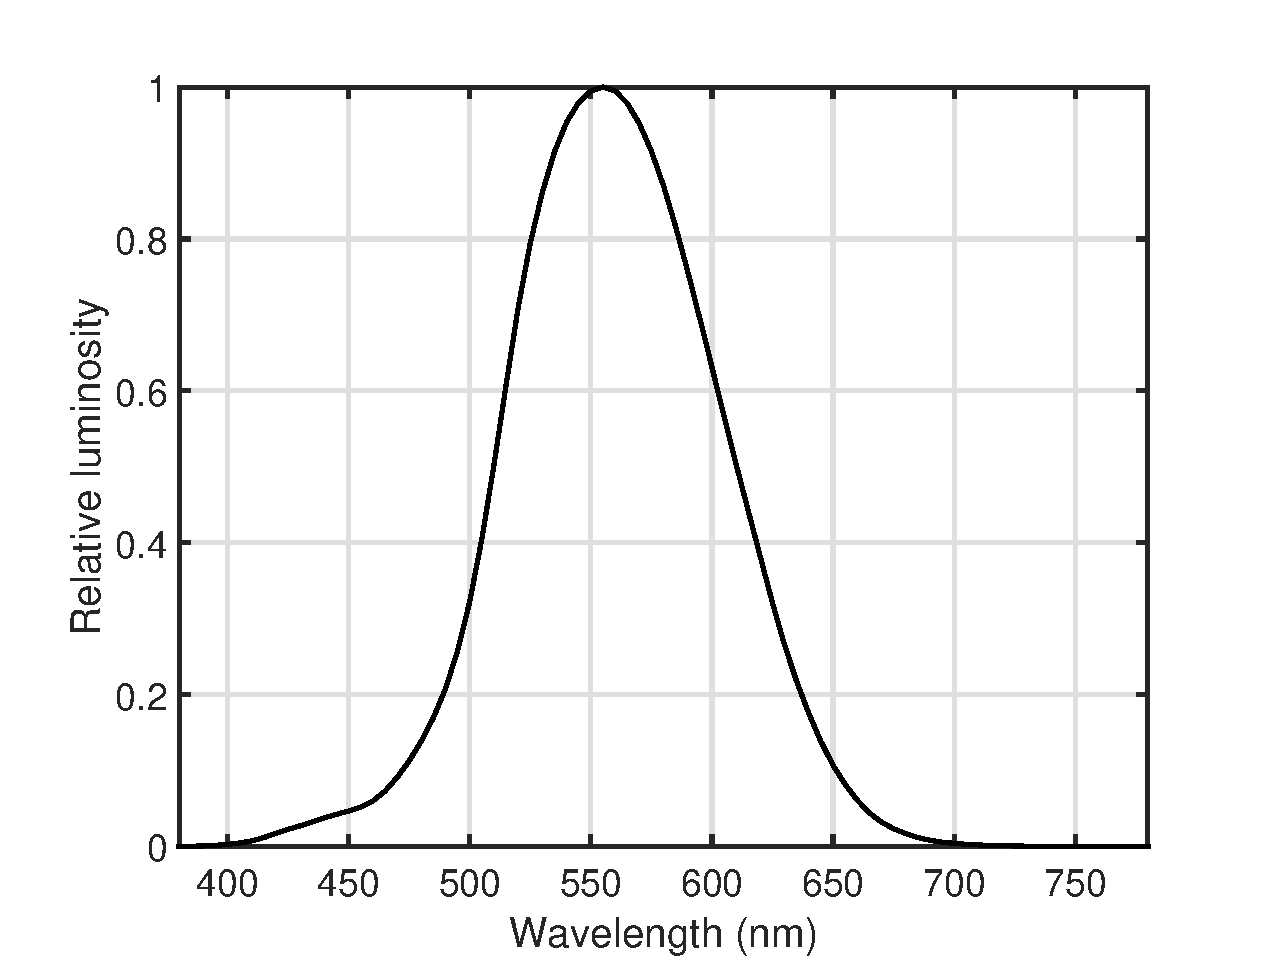
\includegraphics[trim={0.3in 0in 0.75in 0.4in}, clip=true, width=4.25in]{PhotopicResponse2.eps}
	\caption{Typical photopic relative luminous efficiency function}
	\label{figPhotopicCurve}
\end{figure}
The human eye is a sensory organ that enables humans to perceive electromagnetic radiation in a subset of the optical spectrum. \figurename{ \ref{figPhotopicCurve}} \cite{jai89a} shows the typical photopic relative luminous efficiency function of our visual system under moderate to higher levels of illumination. The retina in the eye contains sensory receptors called rods and cones. A normal human eye has three kinds of cones - short (S), medium (M) and long (L) based on the relative wavelengths that induce the peak response. Photons at different wavelengths are absorbed differently by the rods and the three sets of cones. \figurename{ \ref{figConeResp}} \cite{wan96a} shows the normalized absorbance of photons by rods and cones over a range of wavelengths. The peak responses of the cones are 420 nm, 534 nm and 564 nm while that of the rods is 498 nm. Cones are responsible for color vision. Let $S_{i}(\lambda); i\in$ \{S, M, L\}  denote their spectral responses to stimulus over a range of wavelengths. Optical stimulus with an SPD $C(\lambda)$ will induce optical sensation $\alpha_{i}$ within the cones as described in Eq. \eqref{eqAlphaCones}.
\begin{equation}
	\label{eqAlphaCones}
	\alpha_{i} = \int\limits_{0}^{\infty} C(\lambda)S_{i}(\lambda)d\lambda
\end{equation}

\begin{figure}[!t]
	\centering
%		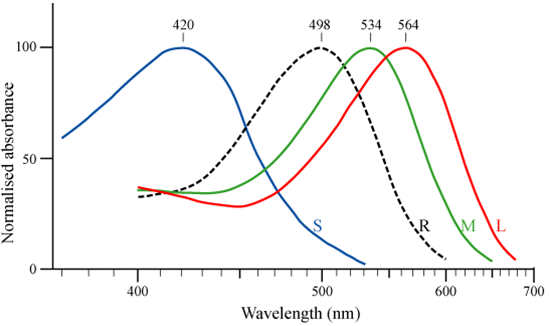
\includegraphics[width=4in]{ConeResponse.png}
    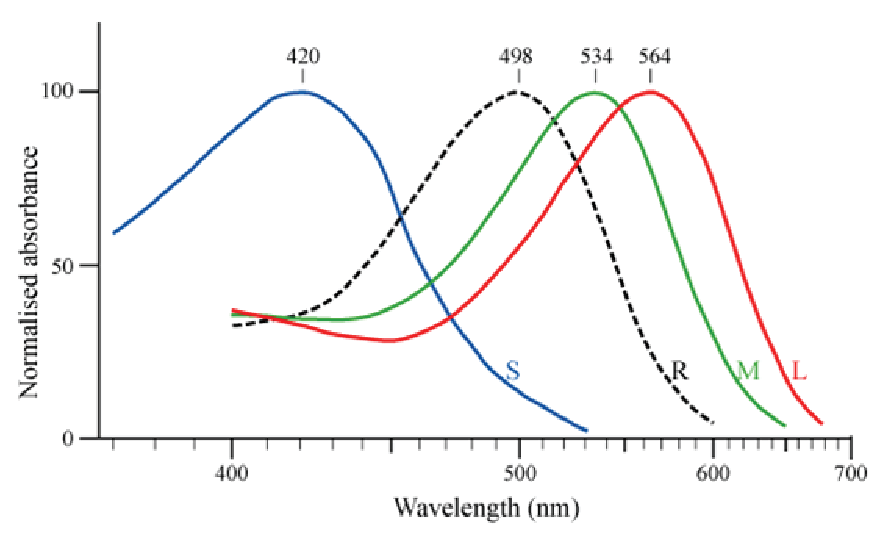
\includegraphics[width=4in]{ConeResponse.eps}
	\caption[Normalized absorbance of photons by rods and cones]{Normalized absorbance of photons by rods and cones \cite{wan96a}}
	\label{figConeResp}
\end{figure}

Grassmann's laws \cite{gra54a} of color matching develop the theory behind the psychovisual color space spanned by cones in the human eye, henceforth called the visual color space (VCS).  This space is a subspace  of the infinite dimensional universal color space (UCS), which contains all possible SPDs. This observation leads to another interpretation of Eq. \eqref{eqAlphaCones} - the point $[{\alpha}_{\text{S}}$, ${\alpha}_{\text{M}}$, ${\alpha}_{\text{L}}]$ is a projection of a given SPD $C(\lambda)$ onto the VCS. Thus it is possible for multiple different SPDs to project onto the same point within the VCS and produce the same sensations, $[{\alpha}_{\text{S}}$, ${\alpha}_{\text{M}}$, ${\alpha}_{\text{L}}]$, in the human eye. These SPDs are sensed as the same color by the human eye and are called metamerically equivalent. Light from three independent primary light sources can be mixed in varying amounts to generate arbitrary colors. Let's call this resulting color space the primary color space (PCS). The projection of the PCS onto the VCS is called the color gamut of the primaries.

Section \ref{subsec:cskNonlinear} provides a mathematical model that incorporates visual perception and maps SPDs to a point on the chromaticity plane. Since metamerically equivalent SPDs generate the same sensation from human eye, they are mapped to the same chromaticity point on the CIE-CS. The color gamut on the CIE-CS is a polygon with chromaticity coordinate of the primary light sources as its vertices.

\section{MM system outline}
\label{subsec:metamericMM}
Metameric modulation (MM) is implemented by using multiple sets of primary light sources capable of providing user requested illumination color.
\begin{figure}[!t]
	\centering
    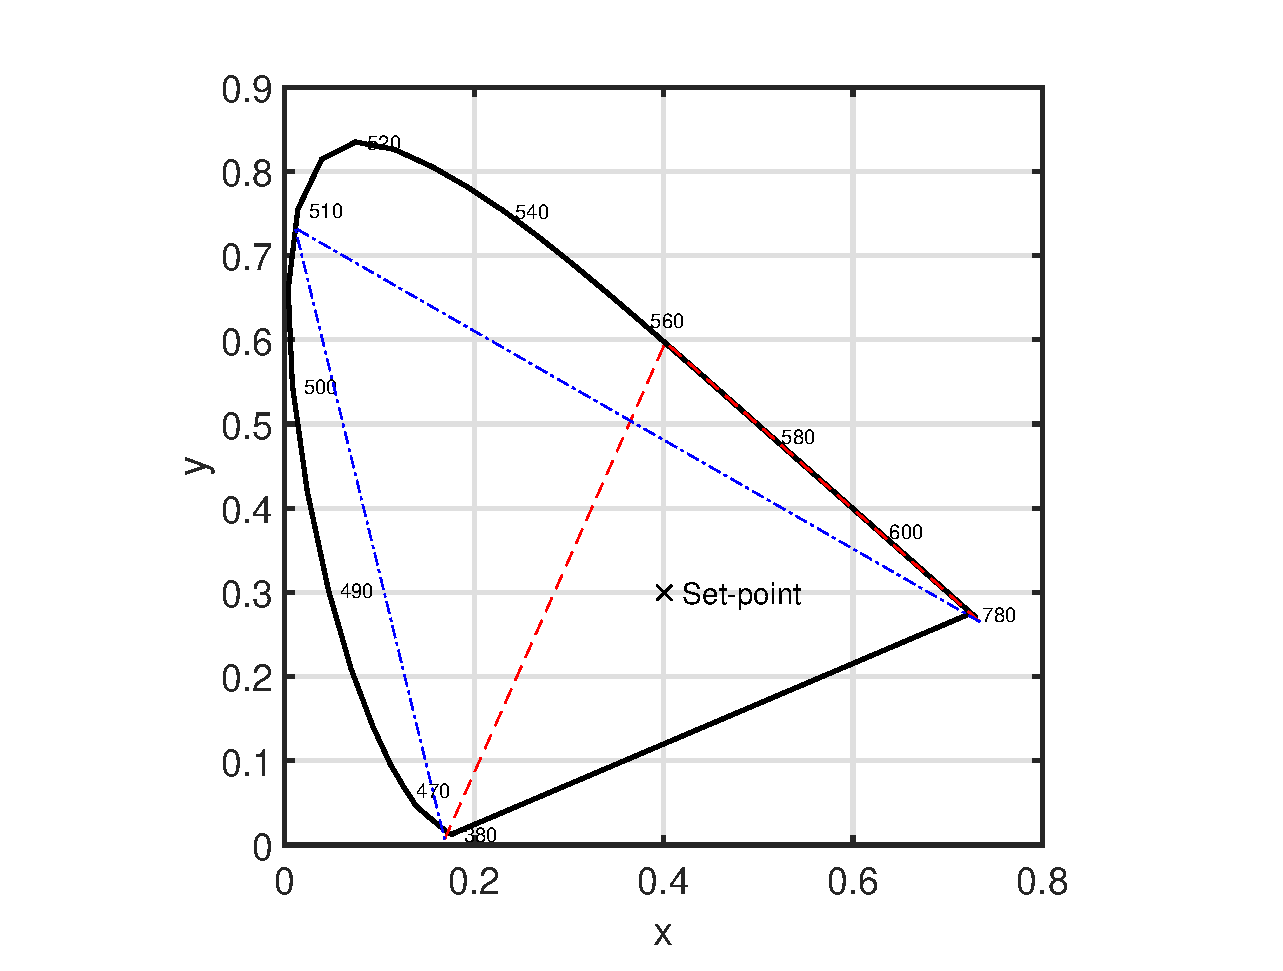
\includegraphics[width=4in]{CIE_XYZ_MM2.eps}
	\caption{Example gamuts for MM with $D=4$, $K=3$ and $M=2$}
	\label{figCIEXYZMM}
\end{figure}
If we have $D$ sources and each primary set is rendered with $K$ primary elements, there are $\binom{D}{K}$ possible primary sets. As the number of primary sets increases, the intersection of their color gamuts quickly approaches an empty set. However only $M$ of the possible primary sets are selected so that the intersection of their color gamuts contain all of the desired lighting states. \figurename{ \ref{figCIEXYZMM}} shows an example for $D=4$, $K=3$ and $M=2$. The two sets of primaries, [Blue, Cyan, Red] and [Blue, Green, Red] have a significant overlap in their color gamuts. In this case they are capable of generating a set point with two different metameric SPDs. 

%\begin{figure}[!t]
	%\centering
%%		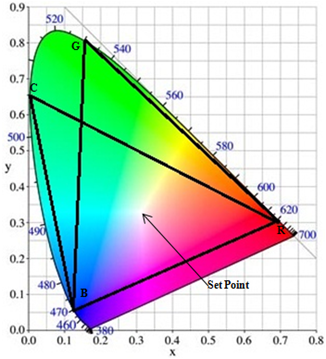
\includegraphics[width=2.5in]{CIE_XYZ_MM.png}
    %
\includegraphics[width=2.5in]{CIE_XYZ_MM.eps}
	%\caption{Example gamuts for MM with $D=4$, $K=3$ and $M=2$}
	%\label{figCIEXYZMM}
%\end{figure}

MM requires detection and discrimination of multiple wavelengths at the receiver. The necessary photodiodes must be designed such that when different primaries are activated to generate a desired ambient color, the receiver can detect which primary set is active while the lighting state appears the same to the human eye. The following derivation details how this can be achieved. 

Consider $K=3$ independent light sources that form one set of primaries. Let each $L_{k}(\lambda)$ be the normalized emission spectra of the $k^{th}$ source such that Eq. \eqref{eqNormEmm} holds.
\begin{equation}
	\label{eqNormEmm}
	\int\limits_{0}^{\infty} L_{k}(\lambda)d\lambda = 1
\end{equation}

Let $\alpha_{i}^{k}$ (\ref{eqAlphaPrimaries}) be the spectral response induced by the $k^{th}$ primary on the $i^{th}$ class of cones.
\begin{equation}
	\label{eqAlphaPrimaries}
	\alpha_{i}^{k} = \int\limits_{0}^{\infty} L_{k}(\lambda)S_{i}(\lambda)d\lambda
\end{equation}

Let $C(\lambda)$ be the SPD of the ambient color that we wish to maintain. Let each $\beta_{k}$ be the amount of the corresponding $L_{k}(\lambda)$ needed to metamerically match $C(\lambda)$. Let $\alpha_{i}^{'}$ (\ref{eqAlphaPrime}) be the aggregate response evoked by the primaries on the $i^{th}$ class of cones. Grassmann's laws of color matching uphold the linearity property of color addition over a wide range of luminances. Our typical ambient illuminance levels lie well within this range of luminances.
\begin{equation}
	\label{eqAlphaPrime}
	\alpha_{i}^{'} = \sum\limits_{k=1}^{K} \beta_{k}\alpha_{i}^{k}
\end{equation}

The primaries must collectively evoke the same spectral responses in the human eye to match the color that is sensed due to $C(\lambda)$. Equating $\alpha_{i}$ in (\ref{eqAlphaCones}) with $\alpha_{i}^{'}$ in (\ref{eqAlphaPrime}) $\forall i$ leads to the color matching equation (\ref{eqColorMatch}). Solving for $\beta_{k}$ gives the relative amount of each primary that is needed to achieve a metamerical match with $C(\lambda)$.
\begin{equation}
	\label{eqColorMatch}
	\sum\limits_{k=1}^{K} \beta_{k}\int\limits_{0}^{\infty} L_{k}(\lambda)S_{i}(\lambda)d\lambda = \int\limits_{0}^{\infty} C(\lambda)S_{i}(\lambda)d\lambda
\end{equation}

Let $W(\lambda)$ be the SPD of the reference white against which the LEDs are calibrated. Let $w_{k}$ be the amount of $L_{k}(\lambda)$ needed to metamerically match $W(\lambda)$. Each tristimulus value, $t_{k}$, of each primary is defined in (\ref{eqTristimulus}). Varying $t_{k}$ for each primary changes the relative amount of the light output from each source that is mixed and thus changes color.
\begin{equation}
	\label{eqTristimulus}
	t_{k} = \beta_{k}/ w_{k}
\end{equation}

Let the individual emission spectra of the $k^{th}$ source from the $m^{th}$ set of primaries be  $L_{k}^{m}(\lambda)$. Now, let us assume we have $P$ receivers selected as mentioned above. Let the effective receiver spectral responses be $S_{p}^{'}(\lambda)$. This includes filter transmittance, concentrator gain and responsivity of the sensor and can be computed similar to Eq. \eqref{eqReff} for a normalized white spectrum. When light from all sources of the $m^{th}$ set of primaries is incident on the $p^{th}$ photodiode, its current output, $I_{p}^{m}$, is given by (\ref{eqPDCurrent}). 
\begin{equation}
	\label{eqPDCurrent}
	I_{p}^{m} = \sum\limits_{k=1}^{K} \beta_{k}\int\limits_{0}^{\infty} L_{k}^{m}(\lambda)S_{p}^{'}(\lambda)d\lambda
\end{equation}

For a given color, the response matrix $R_{g}$ is given by (\ref{eqRespMatrix}). It is possible to design a system where every column of matrix $R_{g}$ would be distinct. One way of achieving this is by using optical filters with their peak transmittance aligned with peak primary source emissions. Optimal estimation of active primary set can be made by comparing output of the photodiodes with the columns of $R_{g}$.
\begin{equation}
	\label{eqRespMatrix}
R_{g} = \left( \begin{array}{ccc}
I_{1}^{1}&\cdots&I_{1}^{M}\\
\vdots&\ddots&\vdots\\
I_{P}^{1}&\cdots&I_{P}^{M}
\end{array} \right)
\end{equation}

\begin{figure}[!t]
	\centering
%		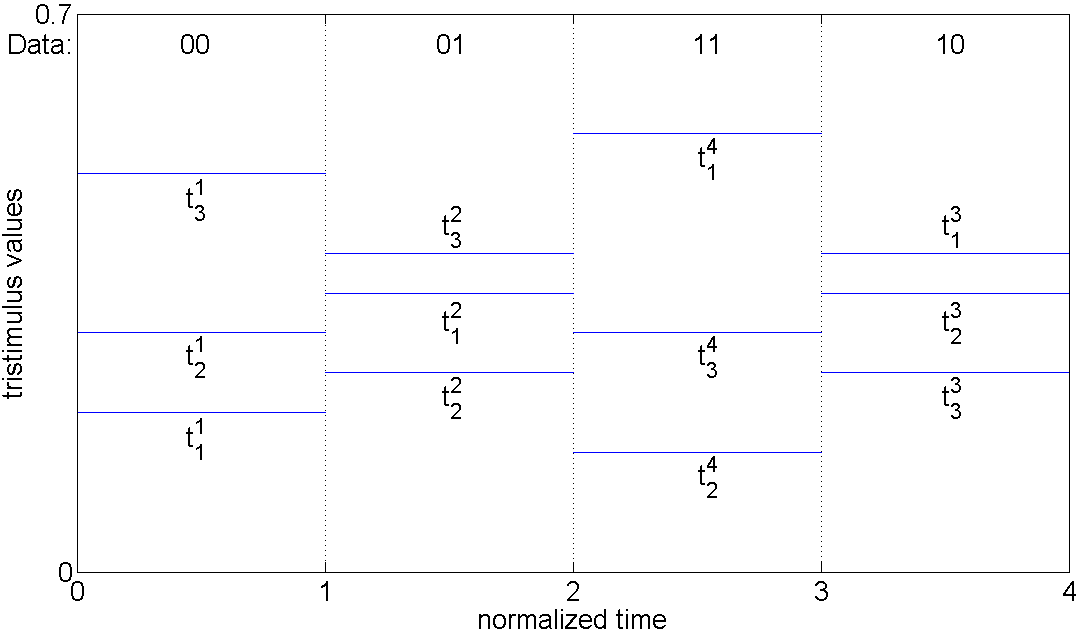
\includegraphics[width=5in]{MM_time.png}
    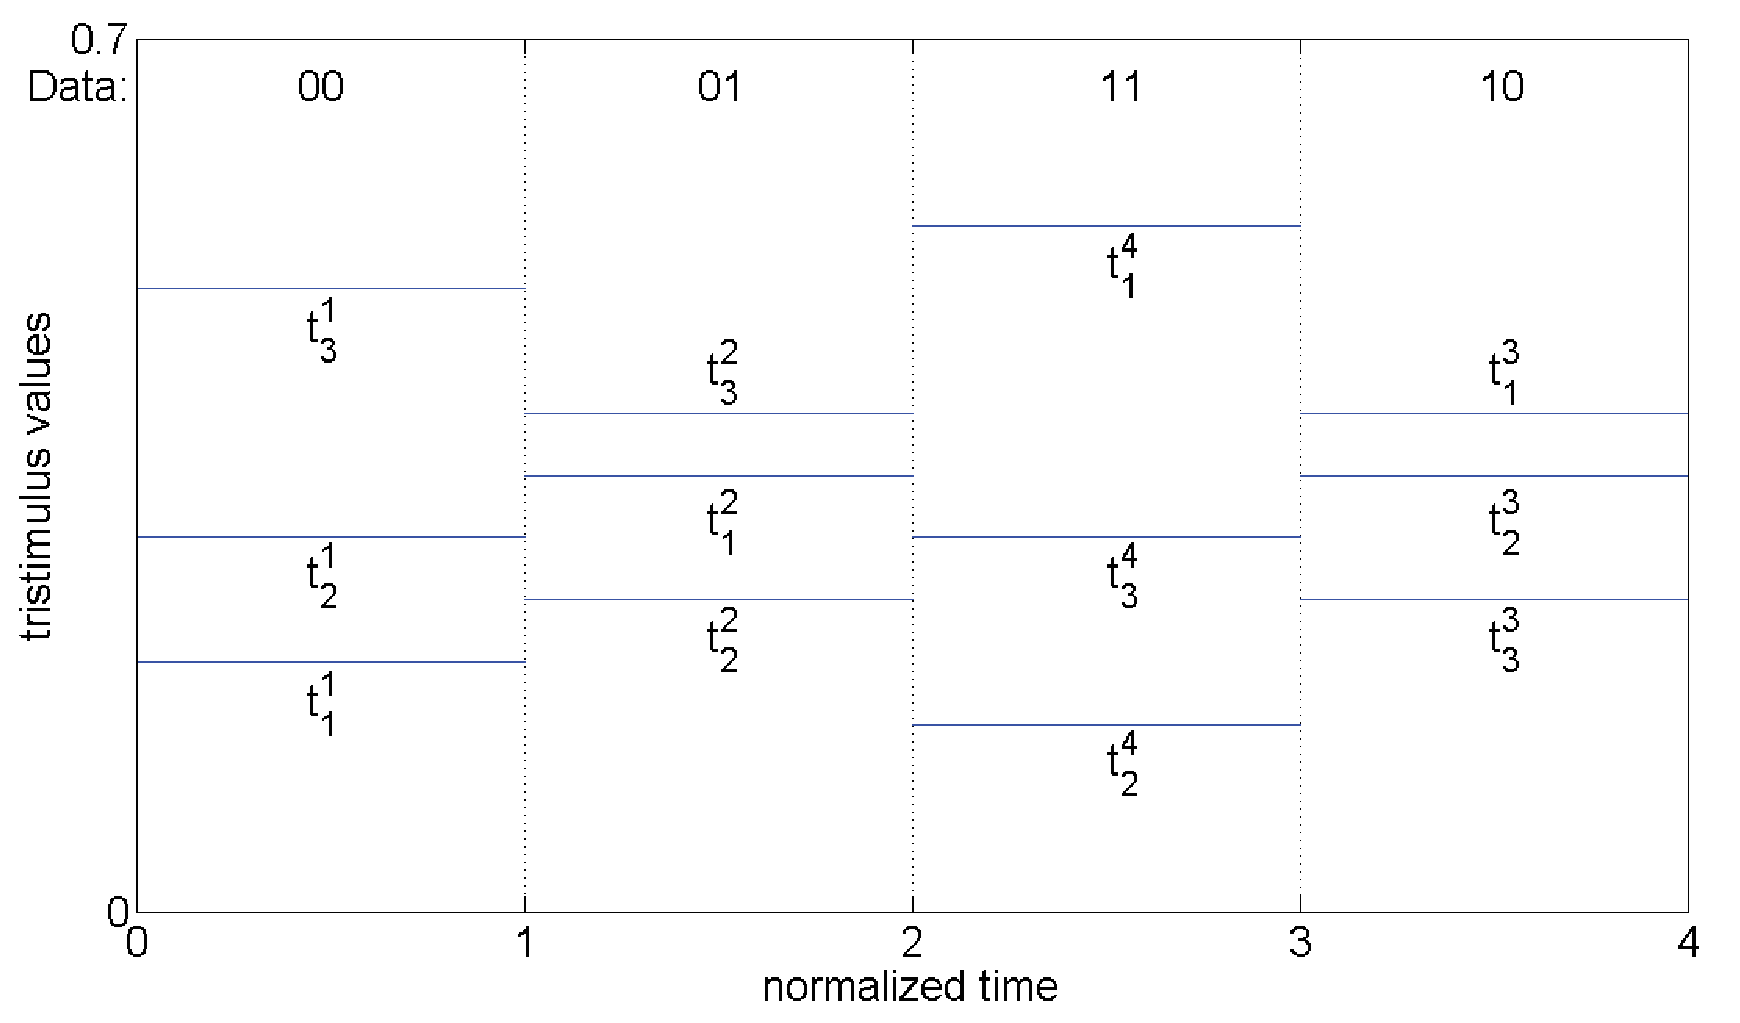
\includegraphics[width=5in]{MM_time.eps}
	\caption[MM example timing diagram]{MM example timing diagram. Illustrates different metamerically equivalent SPDs being transmitted in different time slots.}
	\label{figMMex}
\end{figure}

\begin{table}[!t]
	\centering
		\begin{tabular}{|c|c|}
		\hline
		{Primary Set Index} & {Symbol}\\
		\hline
		1 & 00\\
		2 & 01\\
		3 & 10\\
		4 & 11\\
		\hline
		\end{tabular}
	\caption{MM symbol mapping}
	\label{tblMMSymbol}
\end{table}

The desired ambient lighting state can be specified by a point on the chromaticity plane of the standard CIE-CS. Table \ref{tblMMSymbol} shows example symbol map for $M=4$. CIE-CS color space transforms can then be applied to specify the desired color within the $M$ individual primary sets. Let $t_{k}^{m}$ be the tristimulus value of the $k^{th}$ primary of the $m^{th}$ primary set. These primary sets can now generate distinct but metamerically equivalent SPDs. Switching between the different primary sets transmits symbols.

\figurename{ \ref{figMMex}} illustrates MM using these primary sets to transmit a part of an encoded information stream $(00011110_{2})$. This is accomplished by switching primaries in the order 1-2-4-3. This order can then be detected by analyzing the received signal vector and data can be decoded. The embedded MM modulation is invisible to humans due to metamerism.
%%%%%%%%%%%%%%%%%%%%%%%%%%%%%%%%%%%%%%%%%%%%%%%%%%%%%%%%%%%%%%%%%%%%%%
%%%%%%%%%%%%%%%%%%%%%%%%%%%%%%%%%%%%%%%%%%%%%%%%%%%%%%%%%%%%%%%%%%%%%%
%%%%%%%%%%%%%%%%%%%%%%%%%%%%%%%%%%%%%%%%%%%%%%%%%%%%%%%%%%%%%%%%%%%%%%
\section{MM system performance}
\label{subsec:metamericPerformance}
Performance of MM is studied using color bands and color band combinations as defined in the standard and outlined in section \ref{sec:ieeestd}. Each set of LEDs generating a metameric color point can be implemented as a CBC. Block diagram for MM using CBCs is illustrated in \figurename{ \ref{figMMBD}}. For an $M$-ary MM, log$^{ }_{2}$($M$) bits from the encoded bit--stream are mapped to one out of $M$ possible CBCs. With knowledge of color set--point to generate and user requested illumination level, radiant fluxes $P_{d}; 1\leq d\leq D$ to transmit are calculated. The LED drivers then drive all LEDs to achieve desired illumination color and intensity using the CBC selected by the information to transmit. At the receivers, the incident radiant flux generates electrical signals which are used to estimate transmitted flux $\hat{P}_{d}$ over each type of LED. Using the estimated fluxes, an estimate of active set of LEDs $\hat{\text{CBC}}_{m}$ can be made to recover transmitted information.

\begin{figure}[!t]
	\centering
    
\includegraphics[trim={0in 0in 0in 0in}, clip=true, width=\textwidth]{MMBlockDiagram.png}
	\caption{MM block diagram using IEEE 802.15.7 CBCs}
	\label{figMMBD}
\end{figure}


\figurename{ \ref{figMM_BERvsSNR}} shows BER vs SNR performance for MM for $M$ = 4 and 8. For this analysis, a white chromaticity point of (1/3, 1/3) is generated with the selected CBCs. 4-MM can be implemented with $D$ = 5, 6 or 7. 8-MM is implemented with $D=7$. In absence of illumination constraint, 4-MM achieves the best performance with $D=5$ using CBs from set \{0, 1, 2, 3, 4\} for CBC set \{5, 6, 7, 8\}. Performance plots for 4-MM with $D$ = 6 and 7 are also illustrated for comparison. Implementing 8-MM with CBCs as outlined in IEEE 802.15.7 requires about 60 dB of SNR and seems impractical. However, a different set of LEDs may be used to implement 8-MM to obtain a better performance.

Performance comparison of 4-MM at same illumination intensity level is illustrated in \figurename{ \ref{figMM_BERvsSNR}}. In this case, with $D=5$, 4-MM with CBs from set \{0, 1, 2, 4, 5\} for CBC set \{3, 4, 5, 6\} outperforms others.  CBC set \{5, 6, 7, 8\} has a high luminous efficacy as compared to  CBC set \{3, 4, 5, 6\} and thus is constrained in radiant flux for signaling at a set illumination level. On comparing performance of 4-MM for all possible values of $D$, CBC sets \{1, 2, 4, 5\}, \{1, 2, 4, 6\}, \{1, 2, 4, 7\} and \{1, 2, 4, 8\} with $D=6$ perform the best.
%\afterpage{%
%\clearpage
\begin{figure}[H]
	\centering
		\begin{subfigure}{\textwidth}
		\centering
			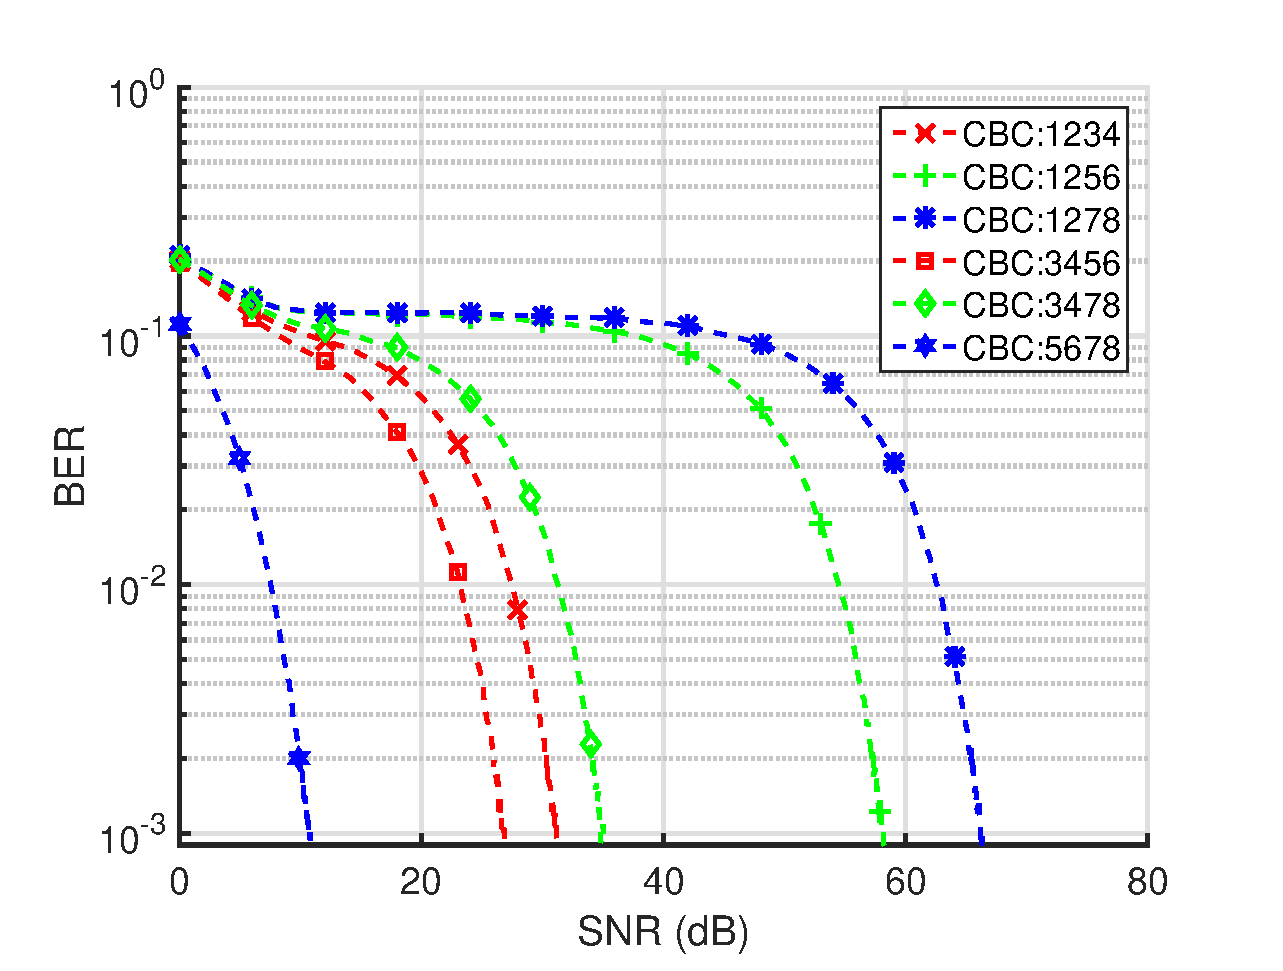
\includegraphics[trim={0.1in 0.0in 0.5in 0.1in}, clip=true, width=0.79\textwidth]{M4_N5_4-MM_BERvsSNR.eps}
			\caption{4-MM, $D$=5}
			\label{fig4MM5}
		\end{subfigure}
		%\hfill
		\begin{subfigure}{\textwidth}
		\centering
			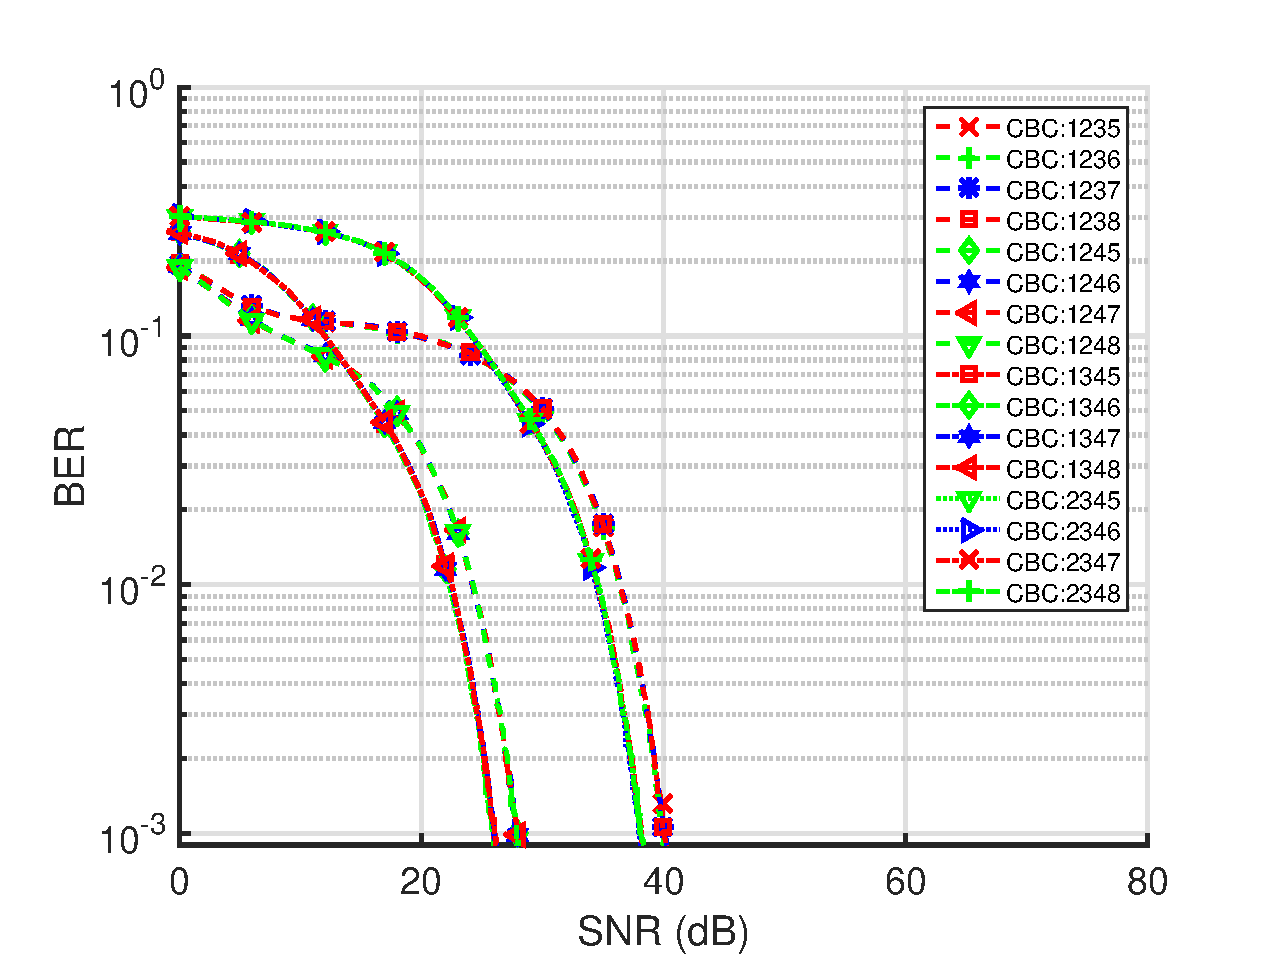
\includegraphics[trim={0.1in 0.0in 0.5in 0.1in}, clip=true, width=0.79\textwidth]{M4_N6_4-MM_BERvsSNR.eps}
			\caption{4-MM, $D$=6}
			\label{fig4MM6}
		\end{subfigure}
		%\vfill
		%\caption{BER vs SNR for different combinations of CBC}
	%\label{figMM_BERvsSNR}
\end{figure}
\begin{figure}[H]
		\ContinuedFloat
		\begin{subfigure}{\textwidth}
		\centering
			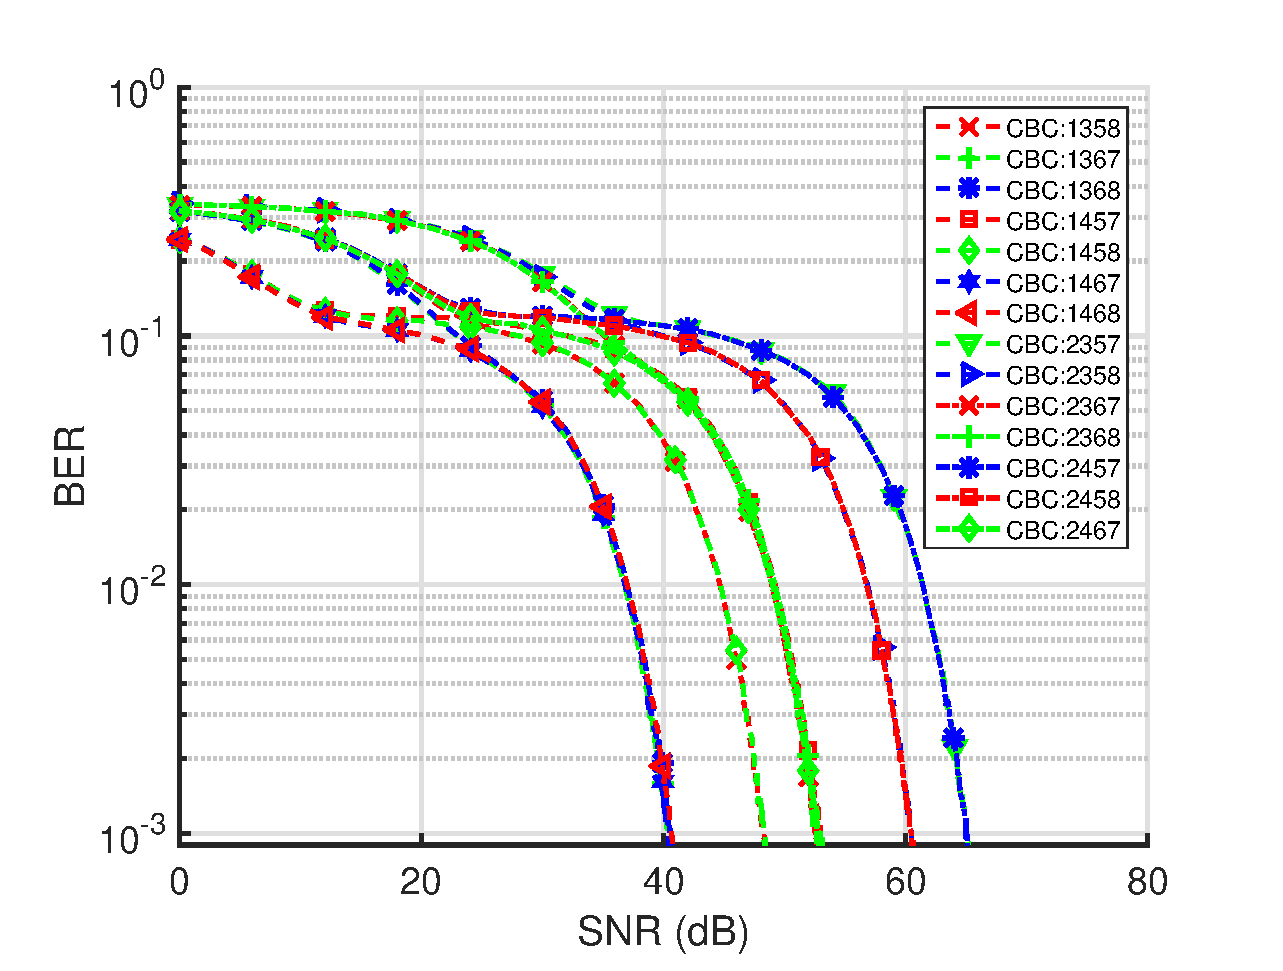
\includegraphics[trim={0.1in 0.0in 0.5in 0.1in}, clip=true, width=0.79\textwidth]{M4_N7_4-MM_BERvsSNR.eps}
			\caption{4-MM, $D$=7}
			\label{fig4MM7}
		\end{subfigure}
		%\hfill
		\begin{subfigure}{\textwidth}
		\centering
			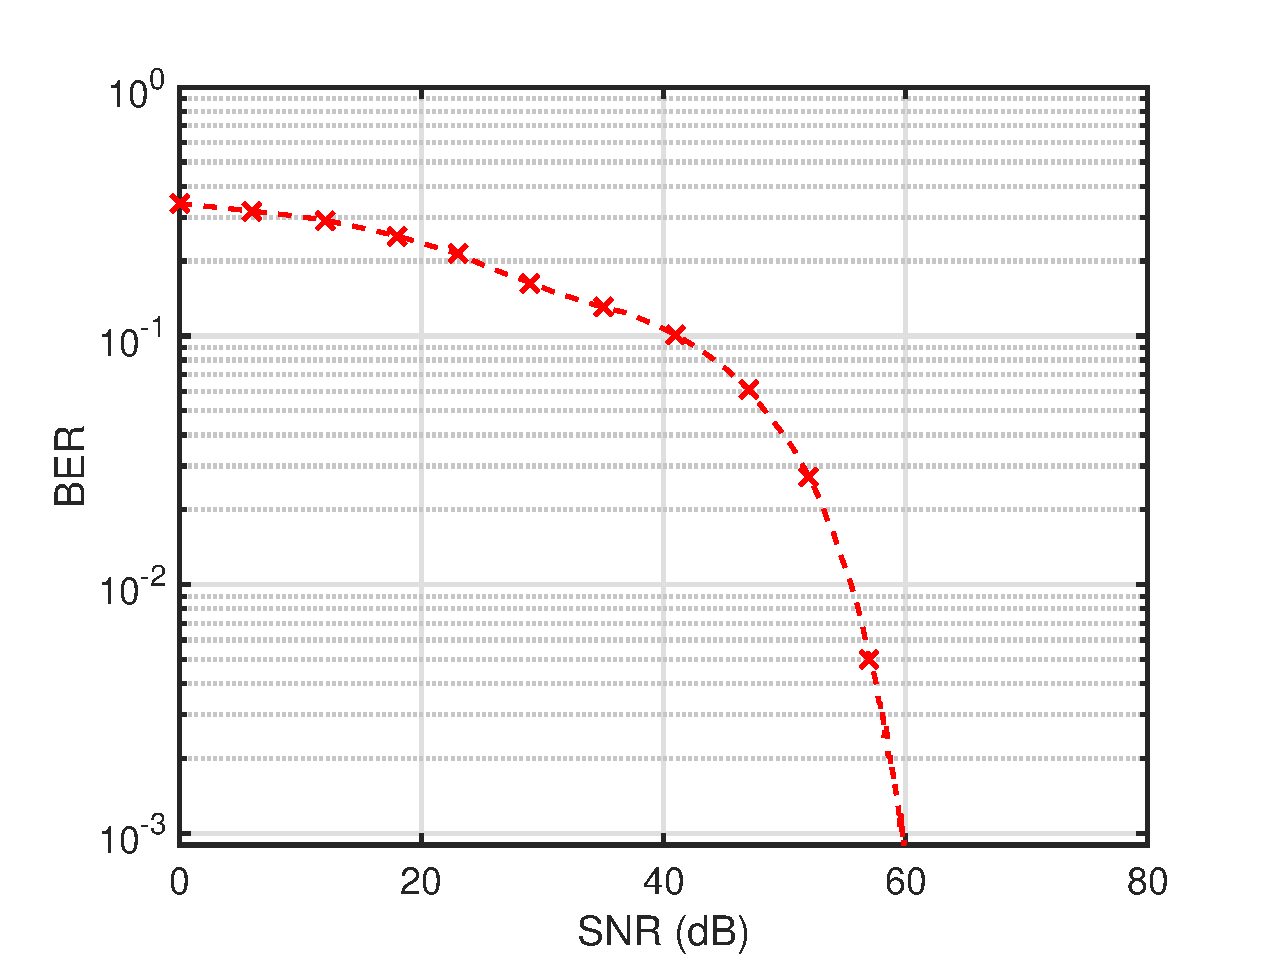
\includegraphics[trim={0.1in 0.0in 0.5in 0.1in}, clip=true, width=0.79\textwidth]{M8_N7_8-MM_BERvsSNR.eps}
			\caption{8-MM, $D$=7}
			\label{fig8MM7}
		\end{subfigure}
	\caption{BER vs SNR for different combinations of CBC}
	\label{figMM_BERvsSNR}
\end{figure}
%\clearpage% Flush page
%}

%\afterpage{%
%\clearpage
\begin{figure}[H]
	\centering
		\begin{subfigure}{\textwidth}
		\centering
			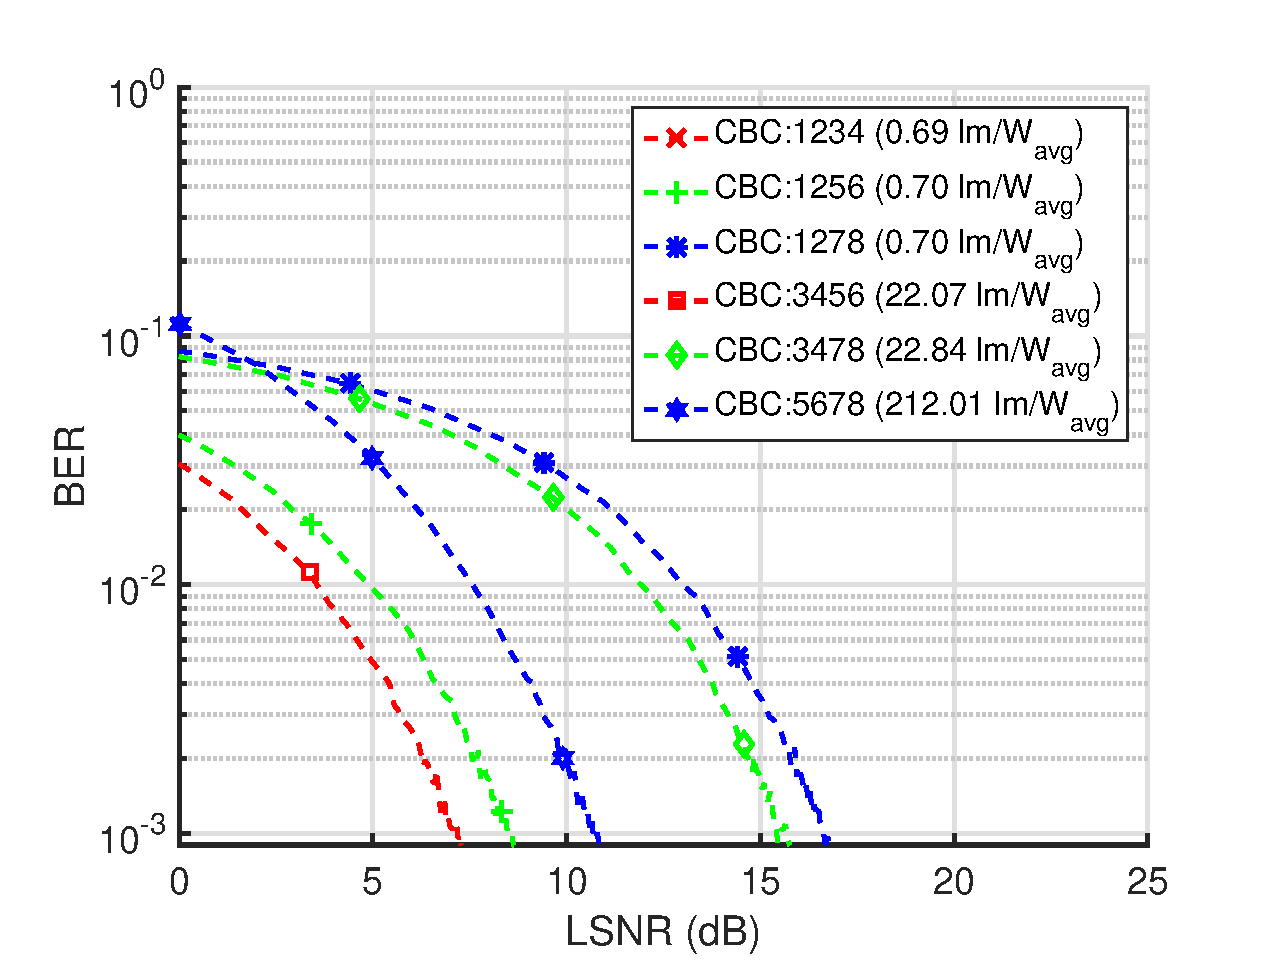
\includegraphics[trim={0.1in 0.0in 0.5in 0.1in}, clip=true, width=0.79\textwidth]{M4_N5_4-MM_BERvsLSNR.eps}
			\caption{4-MM, $D$=5}
			\label{fig4MM5L}
		\end{subfigure}
		%\hfill
		\begin{subfigure}{\textwidth}
		\centering
			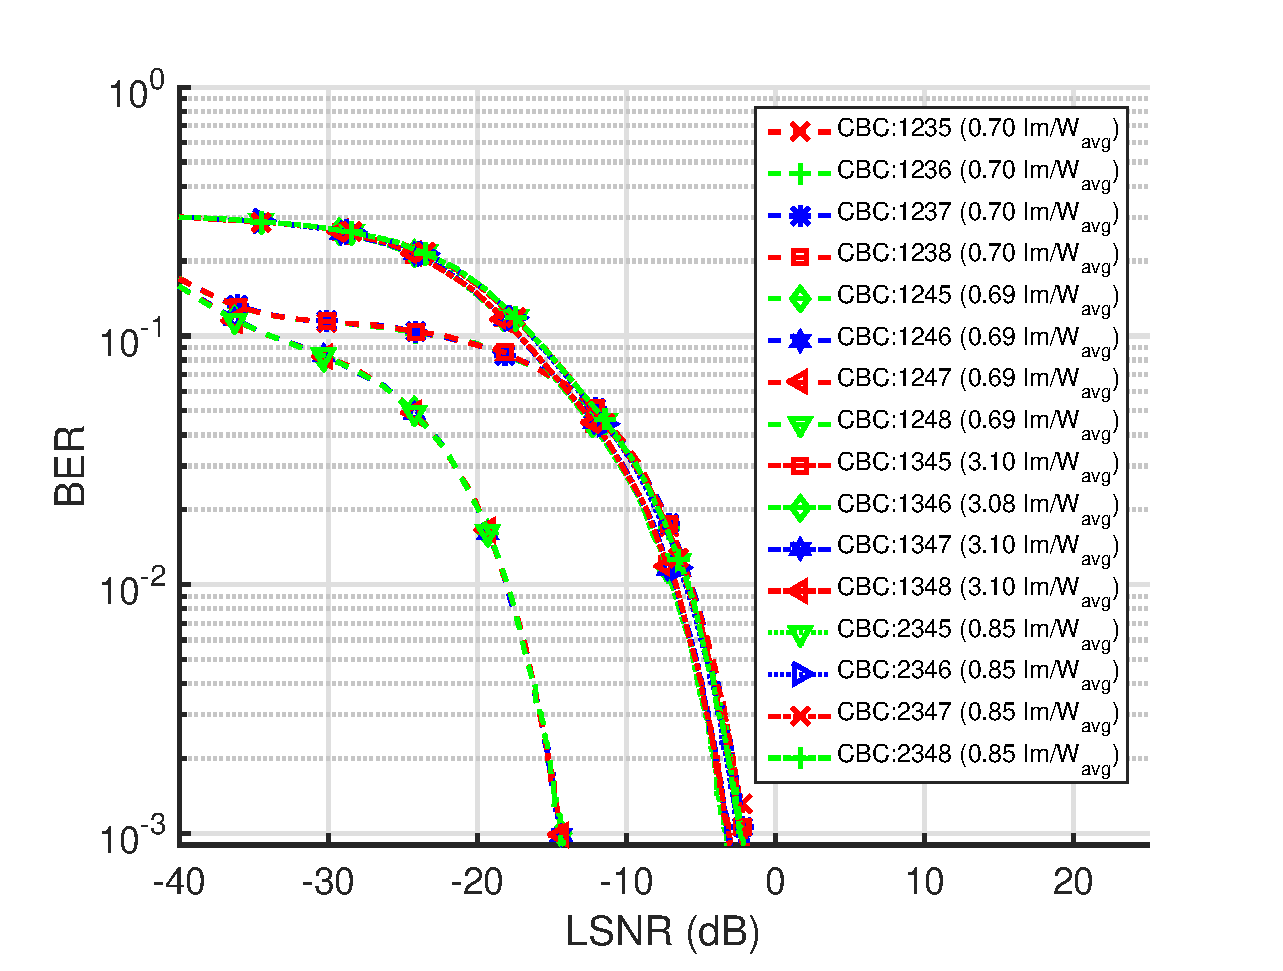
\includegraphics[trim={0.1in 0.0in 0.5in 0.1in}, clip=true, width=0.79\textwidth]{M4_N6_4-MM_BERvsLSNR.eps}
			\caption{4-MM, $D$=6}
			\label{fig4MM6L}
		\end{subfigure}
		%\caption{BER vs LSNR for different combinations of CBC}
	%\label{figMM_BERvsLSNR}
\end{figure}
		%\vfill
\begin{figure}[H]
		\ContinuedFloat
		\begin{subfigure}{\textwidth}
		\centering
			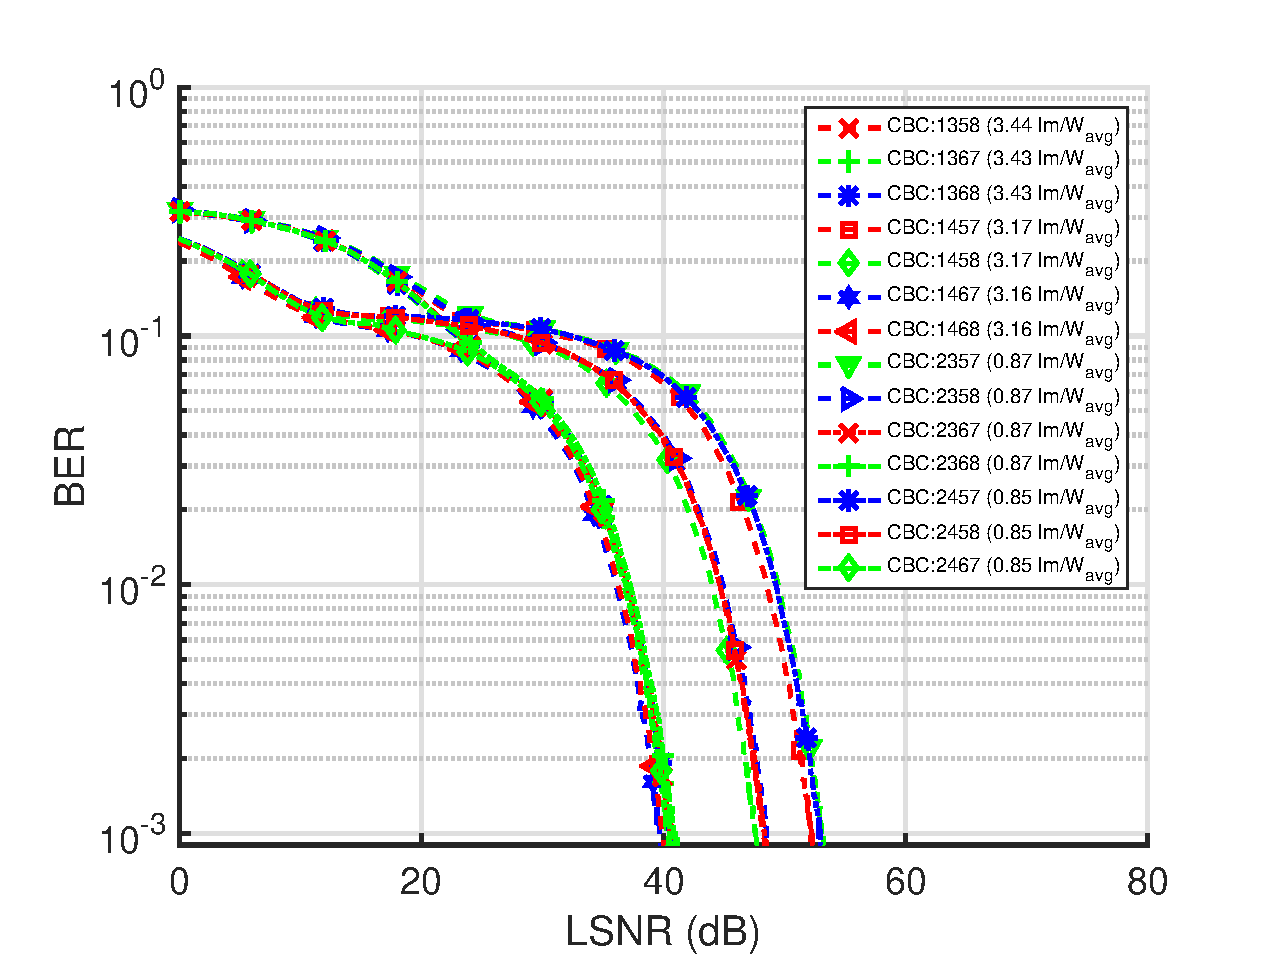
\includegraphics[trim={0.1in 0.0in 0.5in 0.1in}, clip=true, width=0.79\textwidth]{M4_N7_4-MM_BERvsLSNR.eps}
			\caption{4-MM, $D$=7}
			\label{fig4MM7L}
		\end{subfigure}
		%\hfill
		\begin{subfigure}{\textwidth}
		\centering
			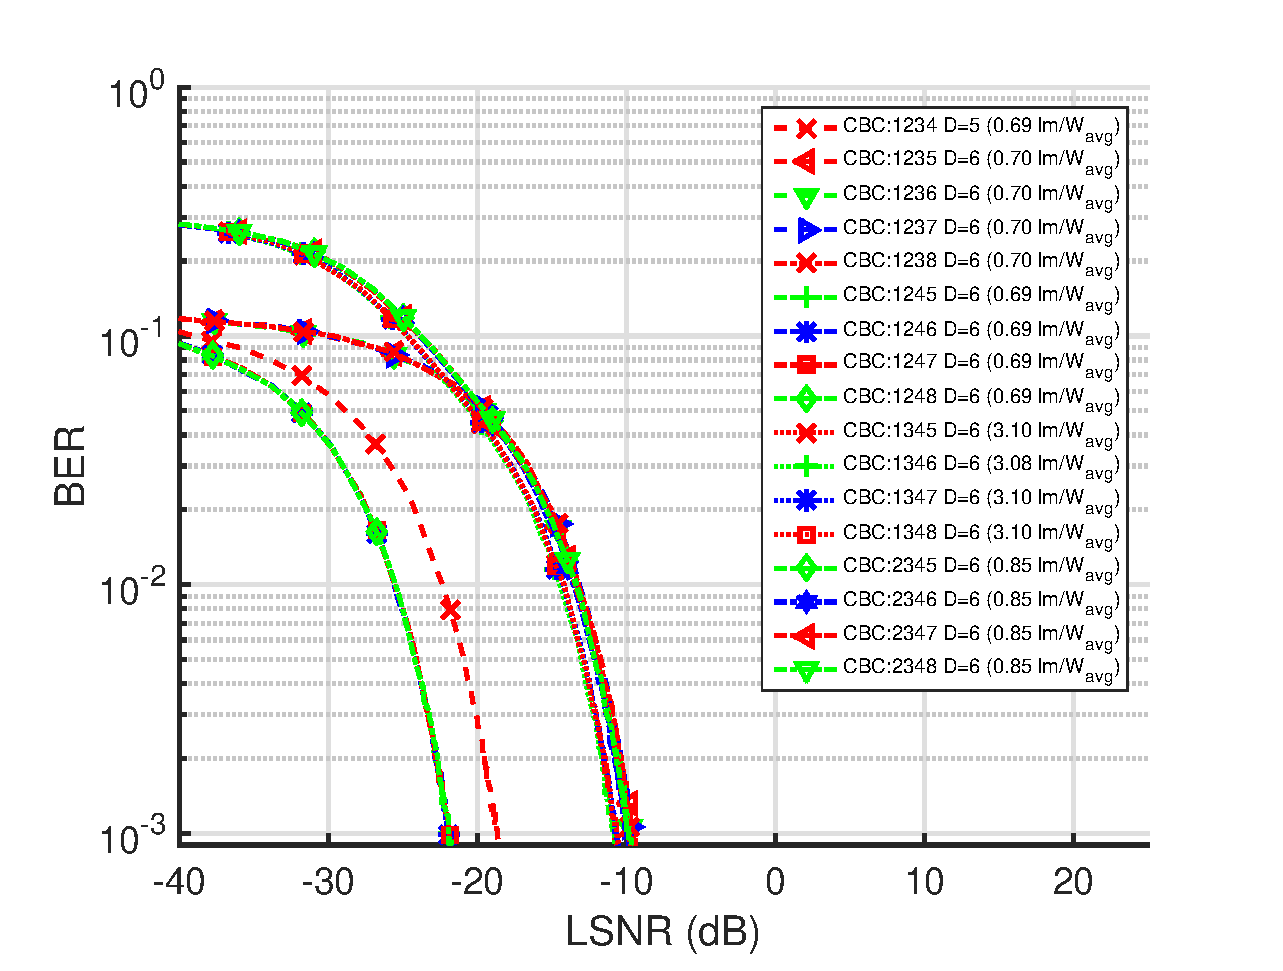
\includegraphics[trim={0.1in 0.0in 0.5in 0.1in}, clip=true, width=0.79\textwidth]{4-MM_BERvsLSNR.eps}
			\caption{4-MM}
			\label{fig4MML}
		\end{subfigure}
	\caption{BER vs LSNR for different combinations of CBC}
	\label{figMM_BERvsLSNR}
\end{figure}
%\clearpage% Flush page
%}

In this chapter, we have proposed MM, a novel modulation scheme for achieving constant color control in optical wireless communication using luminaires. This technique attempts to provide better color rendering for illumination while achieving wireless communication function. MM offers several advantages over CSK. In MM, to generate a set point, we can easily leverage MacAdams ellipses \cite{mac49a} to generate a color at a lower energy consumption point inside each ellipse. Such a technique cannot be applied to CSK because the average then would differ significantly from the set point. Additionally MM always generates the true requested ambient lighting state. The CSK constellation points always generate significantly different colors. Thus MM inherently has the ability to greatly reduce color flicker and improve color rendering. 